\chapter{Käyttötapaukset}

\section{Käyttötapauskaavio}
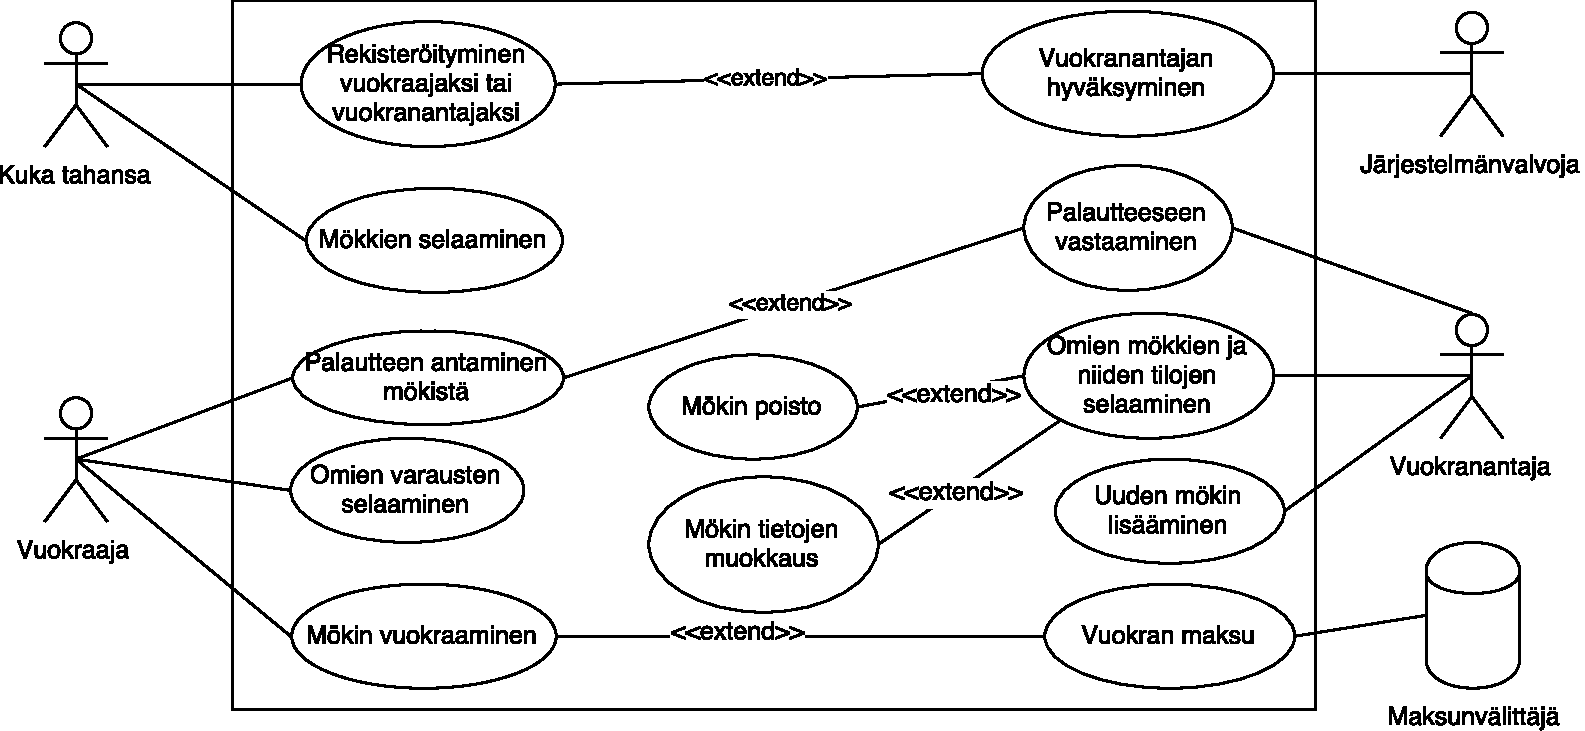
\includegraphics[width = 14cm]{./diagrams/drawio_usecase.pdf}

\section{Käyttäjäryhmät}

\subsection*{Kuka tahansa}
Kenellä tahansa tarkoitetaan kaikkia rekisteröityneitä ja rekisteröitymättömiä käyttäjiä.

\subsection*{Vuokraaja}
Vuokraaja on vuokraajaksi rekisteröitynyt käyttäjä.

\subsection*{Vuokranantaja}
Vuokranantaja on loma-asuntoja vuokralle antava henkilö. Järjestelmänvalvoja hyväksyy uudet vuokranantajat erikseen.

\subsection*{Järjestelmänvalvoja}
Järjestelmänvalvoja huolehtii palvelun moderoinnista ja ylläpitotehtävistä, sekä uusien vuokranantajien hyväksynnästä.

\subsection*{Maksunvälittäjä}
Maksunvälittäjä on ulkopuolinen, automatisoitu maksunvälityspalvelu. Tässä kyseisessä toteutuksessa sitä ei toteuteta.

\section{Käyttötapauskuvaukset}

\subsection{Kirjautumattoman käyttäjän käyttötapaukset}
\subsubsection*{Rekisteröityminen}
Järjestelmään voi rekisteröityä joko vuokraajaksi tai vuokranantajaksi. Vuokraajalta vaaditaan lisätietoja, ja järjestelmänvalvoja hyväksyy uudet vuokraajat käsin. Käyttäjä saa vahvistuksen hyväksynnän jälkeen.
\subsubsection*{Kirjautuminen}

\subsection{Kaikkien käyttäjien käyttötapaukset}
\subsubsection*{Mökkien selaaminen}

\subsection{Vuokraajien käyttötapaukset}
\subsubsection*{Mökin vuokraaminen}
Löydettyään kiinnostavan mökin vuokraaja valitsee vuokrausajankohdan (alku, loppu, kesto) ja näkee, onko mökki saatavilla sinä ajankohtana sekä varauksen hinnan. Jos vuokraaja päättää vuokrata mökin, käyttäjä siirretään maksamaan. Maksun onnistuessa mökki lisätään käyttäjän varauksiin.

\subsubsection*{Varausten selaaminen}
Käyttäjä näkee entiset, nykyiset ja tulevat varaukset.

\subsubsection*{Palautteen antaminen}
Käyttäjä voi antaa palautetta entisistä ja nykyisistä varauksistaan. Palaute voi olla julkista tai vain varaajalle näkyvää.

\subsection{Järjestelmänvalvojan käyttötapaukset}
\subsubsection*{Vuokraajien hyväksyminen}
\subsubsection*{Palautteen moderointi}

\subsection{Vuokranantajan käyttötapaukset}
\subsubsection*{Uuden mökin lisääminen}
Mökkeihin kuuluu nimi, kuvaus, saatavuustiedot ja tiedot varustelusta. Mökkeihin voi liittyä myös kuvia, sijaintidataa yms.
\subsubsection*{Mökkien selaaminen}
\subsubsection*{Mökin tietojen muokkaaminen}
\subsubsection*{Mökin poisto}
\subsubsection*{Palautteeseen vastaaminen}

\subsection{Maksunvälittäjän käyttötapaukset}
\subsubsection*{Vuokranmaksu}
Ulkopuolinen maksunvälittäjä osallistuu vuokranmaksuun pyytämällä käyttäjältä maksutiedot ja välittämällä onnistuneet maksut vuokraajille.